\documentclass[a4paper,10pt]{article}

\usepackage{graphicx}
\usepackage[ansinew]{inputenc}
\usepackage{pdfpages}
\usepackage{listings}
\usepackage[spanish]{babel}

\definecolor{Cgreen}{rgb}{0,0.6,0}
\definecolor{Cgray}{rgb}{0.5,0.5,0.5}
\definecolor{Cpurple}{rgb}{0.58,0,0.82}
\definecolor{Cwhite}{rgb}{255,255,255}

\lstdefinestyle{CStyle}{
    backgroundcolor=\color{Cwhite},   
    commentstyle=\color{Cgreen},
    keywordstyle=\color{magenta},
    numberstyle=\tiny\color{Cgray},
    stringstyle=\color{Cpurple},
    basicstyle=\footnotesize,
    breakatwhitespace=false,         
    breaklines=true,                 
    captionpos=b,                    
    keepspaces=true,                 
    numbers=left,                    
    numbersep=5pt,                  
    showspaces=false,                
    showstringspaces=false,
    showtabs=false,                  
    tabsize=2,
    language=C
}

\title{\textbf{Trabajo Pr�ctico N� 2: Memorias cache}}

\author{
	Sebastian Ripari, \textit{Padr�n Nro. 96.453}\\
	\texttt{sebastiandanielripari@hotmail.com}\\[2.5ex]
	Cesar Emanuel Lencina, \textit{Padr�n Nro. 96.078}\\
	\texttt{cesar\char`_1990@live.com}\\[2.5ex]
	Pablo Sivori, \textit{Padr�n Nro. 84.026}\\
	\texttt{sivori.daniel@gmail.com}\\[2.5ex]
	\normalsize{2do. Cuatrimestre de 2017}\\
	\normalsize{66.20 Organizaci�n de Computadoras  $-$ Pr�ctica Jueves}\\
	\normalsize{Facultad de Ingenier�a, Universidad de Buenos Aires}\\
}

\date{}

\begin{document}

\maketitle
\thispagestyle{empty}   % quita el n�mero en la primer p�gina

\begin{abstract}
Se implemento un programa que simula una memoria cache asociativa por conjuntos de dos vias, de 4 KB de capacidad, bloques de 32 bytes, politica de reemplazo LRU y politica de escritura WB/WA. Y una memoria principal con un tamano de 64KB. Con el objetivo de simular el funcionamiento de la memoria cache, es decir el trabajo de traerse los datos de memoria principal cuando estos van siendo utilizados.
\end{abstract}

\null\newpage

\tableofcontents

\null\newpage

\section{Introducci�n}

La memoria cache, se encuentra en un nivel de la jerarquia de memoria, que tiene la caracteristica de ser mas rapido que la memoria principal y mas lento que los registros del procesador. Su tama�o es muy inferior al de la memoria principal, por lo tanto la informacion que se traiga debera ser la que mas se use, para asi evitar lo mas posible el uso de la memoria pricipal.

\section{Desarrollo}

Mediante el lenguaje de programacion C, se llevo a cabo un tipo de dato abstracto (TDA) que simula la estructura y la logica/funcionamiento de una memoria cache con las caracteristicas especificadas en el enunciado. Y ademas tambien se llevo a cabo un TDA que simula una memoria principal.

\subsection{TDA: memoria\_cache\_t}

\subsubsection{Estructura de datos}
Este TDA, contiene un array de conjuntos, para representar el dato conjunto se creo el TDA llamado set\_t. Este a su ves tiene un array de bloques, que para representar el bloque se creo el TDA block\_t, que a su ves este tiene un array de bytes, que son las palabras que contiene el bloque. Me parecio oportuna la idea de crear TDAs para lograr de forma clara lo que es la estructura de datos de esta memoria cache. Que se vean claramente sus componentes y tambien lograr un amigable acceso.

\subsubsection{Metodos} 

\textbf{void memory\_cache\_init(memory\_cache\_t *self) :} 
Se encarga de inicializar el flag valid en 0 que significa "valido", y el flag dirty en 0 que significa "no dirty" de todos los bloques de la cache.\newline

\textbf{int memory\_cache\_read\_byte(memory\_cache\_t *self, unsigned short int address) :}
Mediante el address, se hace una descomposicion de este en los campos tag, set y word, y con estos se hace una busqueda del dato en la cache, sino es encontrado se lleva de memoria principal a cache el bloque que contenga este dato. Pero en este caso la funcion devolvera -1. En cambio si el dato si estaba, lo devuelve.\newline

\textbf{int memory\_cache\_write\_byte(memory\_cache\_t *self, unsigned short int address, unsigned char value) :}
Mediante el address, se hace una descomposicion de este en los campos tag, set y word, y con estos se hace una busqueda del dato en la cache para escribirlo, sino es encontrdo se lleva de memoria principal a cache el bloque que contenga este dato.  Pero en este caso la funcion devolera -1. En cambio si el bloque estaba, devuelve 0.\newline

\textbf{float memory\_cache\_get\_miss\_rate(memory\_cache\_t *self) :}
Este metodo realiza el calculo del miss rate, haciendo la simple division de los atributos almacenados en el TDA memory\_cache\_t, estos son n\_misses y n\_reads.\newline

\subsection{TDA: memoria\_principal\_t}

\subsubsection{Estructura de datos}
Simplemente es un array de bytes.

\subsubsection{Metodos}
\textbf{void memory\_principal\_init(memory\_principal\_t *self) :}

Se encarga de incializar todas las palabras en 0.

\textbf{void memory\_principal\_get\_block(memory\_principal\_t *self, unsigned int address, char *bytes, int n\_bytes) :}

Devuelve un bloque de bytes de tama�o de n\_bytes, en la dirreccion pedida, es decir address.

\textbf{void memory\_principal\_set\_block(memory\_principal\_t *self, unsigned int address, unsigned char *bytes, int n\_bytes) :}

Setea un bloque de bytes de tama�o de n\_bytes, en la dirreccion pedida, es decir address.

\null\newpage

\section{Instrucciones de compilacion}
La compilacion se realiza simplemente utilizando el comando:\newline
\textbf{make}\newline
Acto seguido se creara un ejecutable llamado tp.\newline

\section{Mediciones}

\textbf{./tp test\_files/prueba1.mem\newline}
\verb|R 0 -> (set: 0, tag: 0, word: 0) MISS|\newline
\verb|R 4096 -> (set: 0, tag: 2, word: 0) MISS|\newline
\verb|R 8 -> (set: 0, tag: 0, word: 8) HIT: el dato es 0|\newline
\verb|R 4100 -> (set: 0, tag: 2, word: 4) HIT: el dato es 0|\newline
\verb|R 8192 -> (set: 0, tag: 4, word: 0) MISS|\newline
\verb|W 4096, 228 -> (set: 0, tag: 2, word: 0) HIT|\newline
\verb|W 4097, 255 -> (set: 0, tag: 2, word: 1) HIT|\newline
\verb|W 4098, 1 -> (set: 0, tag: 2, word: 2) HIT|\newline
\verb|R 4096 -> (set: 0, tag: 2, word: 0) HIT: el dato es 228|\newline
\verb|Number of misses: 3|\newline
\verb|Number of references: 9|\newline
\verb|Miss rate: 0.333333|\newline

\textbf{./tp test\_files/prueba2.mem\newline}
\verb|R 0 -> (set: 0, tag: 0, word: 0) MISS|\newline
\verb|R 31 -> (set: 0, tag: 0, word: 31) HIT: el dato es 0|\newline
\verb|W 32, 10 -> (set: 1, tag: 0, word: 0) MISS|\newline
\verb|R 32 -> (set: 1, tag: 0, word: 0) HIT: el dato es 10|\newline
\verb|W 32, 20 -> (set: 1, tag: 0, word: 0) HIT|\newline
\verb|R 32 -> (set: 1, tag: 0, word: 0) HIT: el dato es 20|\newline
\verb|R 4128 -> (set: 1, tag: 2, word: 0) MISS|\newline
\verb|R 8223 -> (set: 0, tag: 4, word: 31) MISS|\newline
\verb|R 32 -> (set: 1, tag: 0, word: 0) HIT: el dato es 20|\newline
\verb|R 32 -> (set: 1, tag: 0, word: 0) HIT: el dato es 20|\newline
\verb|Number of misses: 4|\newline
\verb|Number of reads: 10|\newline
\verb|Miss rate: 0.400000|\newline

\textbf{./tp test\_files/prueba3.mem\newline}
\verb|W 0, 1 -> (set: 0, tag: 0, word: 0) MISS|\newline
\verb|W 1, 2 -> (set: 0, tag: 0, word: 1) HIT|\newline
\verb|W 2, 3 -> (set: 0, tag: 0, word: 2) HIT|\newline
\verb|W 3, 4 -> (set: 0, tag: 0, word: 3) HIT|\newline
\verb|W 4, 5 -> (set: 0, tag: 0, word: 4) HIT|\newline
\verb|R 0 -> (set: 0, tag: 0, word: 0) HIT: el dato es 1|\newline
\verb|R 1 -> (set: 0, tag: 0, word: 1) HIT: el dato es 2|\newline
\verb|R 2 -> (set: 0, tag: 0, word: 2) HIT: el dato es 3|\newline
\verb|R 3 -> (set: 0, tag: 0, word: 3) HIT: el dato es 4|\newline
\verb|R 4 -> (set: 0, tag: 0, word: 4) HIT: el dato es 5|\newline
\verb|Number of misses: 1|\newline
\verb|Number of reads: 10|\newline
\verb|Miss rate: 0.100000|\newline

\textbf{./tp test\_files/prueba4.mem\newline}
\verb|W 0, 1 -> (set: 0, tag: 0, word: 0) MISS|\newline
\verb|W 1, 2 -> (set: 0, tag: 0, word: 1) HIT|\newline
\verb|W 2, 3 -> (set: 0, tag: 0, word: 2) HIT|\newline
\verb|W 3, 4 -> (set: 0, tag: 0, word: 3) HIT|\newline
\verb|W 4, 5 -> (set: 0, tag: 0, word: 4) HIT|\newline
\verb|R 0 -> (set: 0, tag: 0, word: 0) HIT: el dato es 1|\newline
\verb|R 1 -> (set: 0, tag: 0, word: 1) HIT: el dato es 2|\newline
\verb|R 2 -> (set: 0, tag: 0, word: 2) HIT: el dato es 3|\newline
\verb|R 3 -> (set: 0, tag: 0, word: 3) HIT: el dato es 4|\newline
\verb|R 4 -> (set: 0, tag: 0, word: 4) HIT: el dato es 5|\newline
\verb|R 4096 -> (set: 0, tag: 2, word: 0) MISS|\newline
\verb|R 8192 -> (set: 0, tag: 4, word: 0) MISS|\newline
\verb|R 0 -> (set: 0, tag: 0, word: 0) MISS|\newline
\verb|R 1 -> (set: 0, tag: 0, word: 1) HIT: el dato es 2|\newline
\verb|R 2 -> (set: 0, tag: 0, word: 2) HIT: el dato es 3|\newline
\verb|R 3 -> (set: 0, tag: 0, word: 3) HIT: el dato es 4|\newline
\verb|R 4 -> (set: 0, tag: 0, word: 4) HIT: el dato es 5|\newline
\verb|Number of misses: 4|\newline
\verb|Number of reads: 17|\newline
\verb|Miss rate: 0.235294|\newline

\textbf{./tp test\_files/prueba5.mem\newline}
\verb|R 0 -> (set: 0, tag: 0, word: 0) MISS|\newline
\verb|R 4096 -> (set: 0, tag: 2, word: 0) MISS|\newline
\verb|R 8192 -> (set: 0, tag: 4, word: 0) MISS|\newline
\verb|R 4096 -> (set: 0, tag: 2, word: 0) HIT: el dato es 0|\newline
\verb|R 0 -> (set: 0, tag: 0, word: 0) MISS|\newline
\verb|R 4096 -> (set: 0, tag: 2, word: 0) HIT: el dato es 0|\newline
\verb|Number of misses: 4|\newline
\verb|Number of reads: 6|\newline
\verb|Miss rate: 0.666667|\newline

\null\newpage

\section{Conclusiones}

La primera conclucion a la que llegamos es lo importante de que cuando se necesita el byte de una palabra, no solo se lleve esa palabra a cache, sino todo el bloque que comprende a esa palabra, esto trae en la mayoria de los casos una gran optimizacion, el caso mas facil de ver esto es en un vector, usualmente no solo nos interesa un valor de un vector, sino los valores de todo el vector, y como esta informacion esta contigua en memoria, el cache en el momento de agarrar esa informacion agarraria la de todo el vector o gran parte del vector.

Y lo segundo que logramos ver, es que los caches que se estructuran por conjuntos, son bastante rapidos por tener el indexado del conjuntos, pero por ejemplo en este caso que al ser de dos bloques por conjunto, su asociatividad es bastante baja, y esto produce que los bloques se reemplacen mucho mas que si por ejemplo fuera un cache totalmente asociativo, es decir que todos los bloques estuvieran dentro de un solo conjunto. Pero bueno esto es un trade of entre velocidad de match del bloque y bajar la cantidad de misses.

\begin{thebibliography}{99}

\bibitem{wikipedia} Cache (Informatica), https://es.wikipedia.org/wiki/Cach

\bibitem{ajbeas} Apunte, http://ajbeas.webcindario.com/asocon.html

\end{thebibliography}

\newpage

\section{Codigo fuente del programa en C:}

\newpage
{\huge{main.c}}
\lstinputlisting[style=CStyle]{main.c}

\newpage
{\huge{memory\_cache.c}}
\lstinputlisting[style=CStyle]{memory_cache.h}

\newpage
{\huge{memory\_cache.h}}
\lstinputlisting[style=CStyle]{memory_cache.c}

\newpage
{\huge{memory\_principal.c}}
\lstinputlisting[style=CStyle]{memory_principal.h}

\newpage
{\huge{memory\_principal.h}}
\lstinputlisting[style=CStyle]{memory_principal.c}

\newpage

\section{Enunciado}

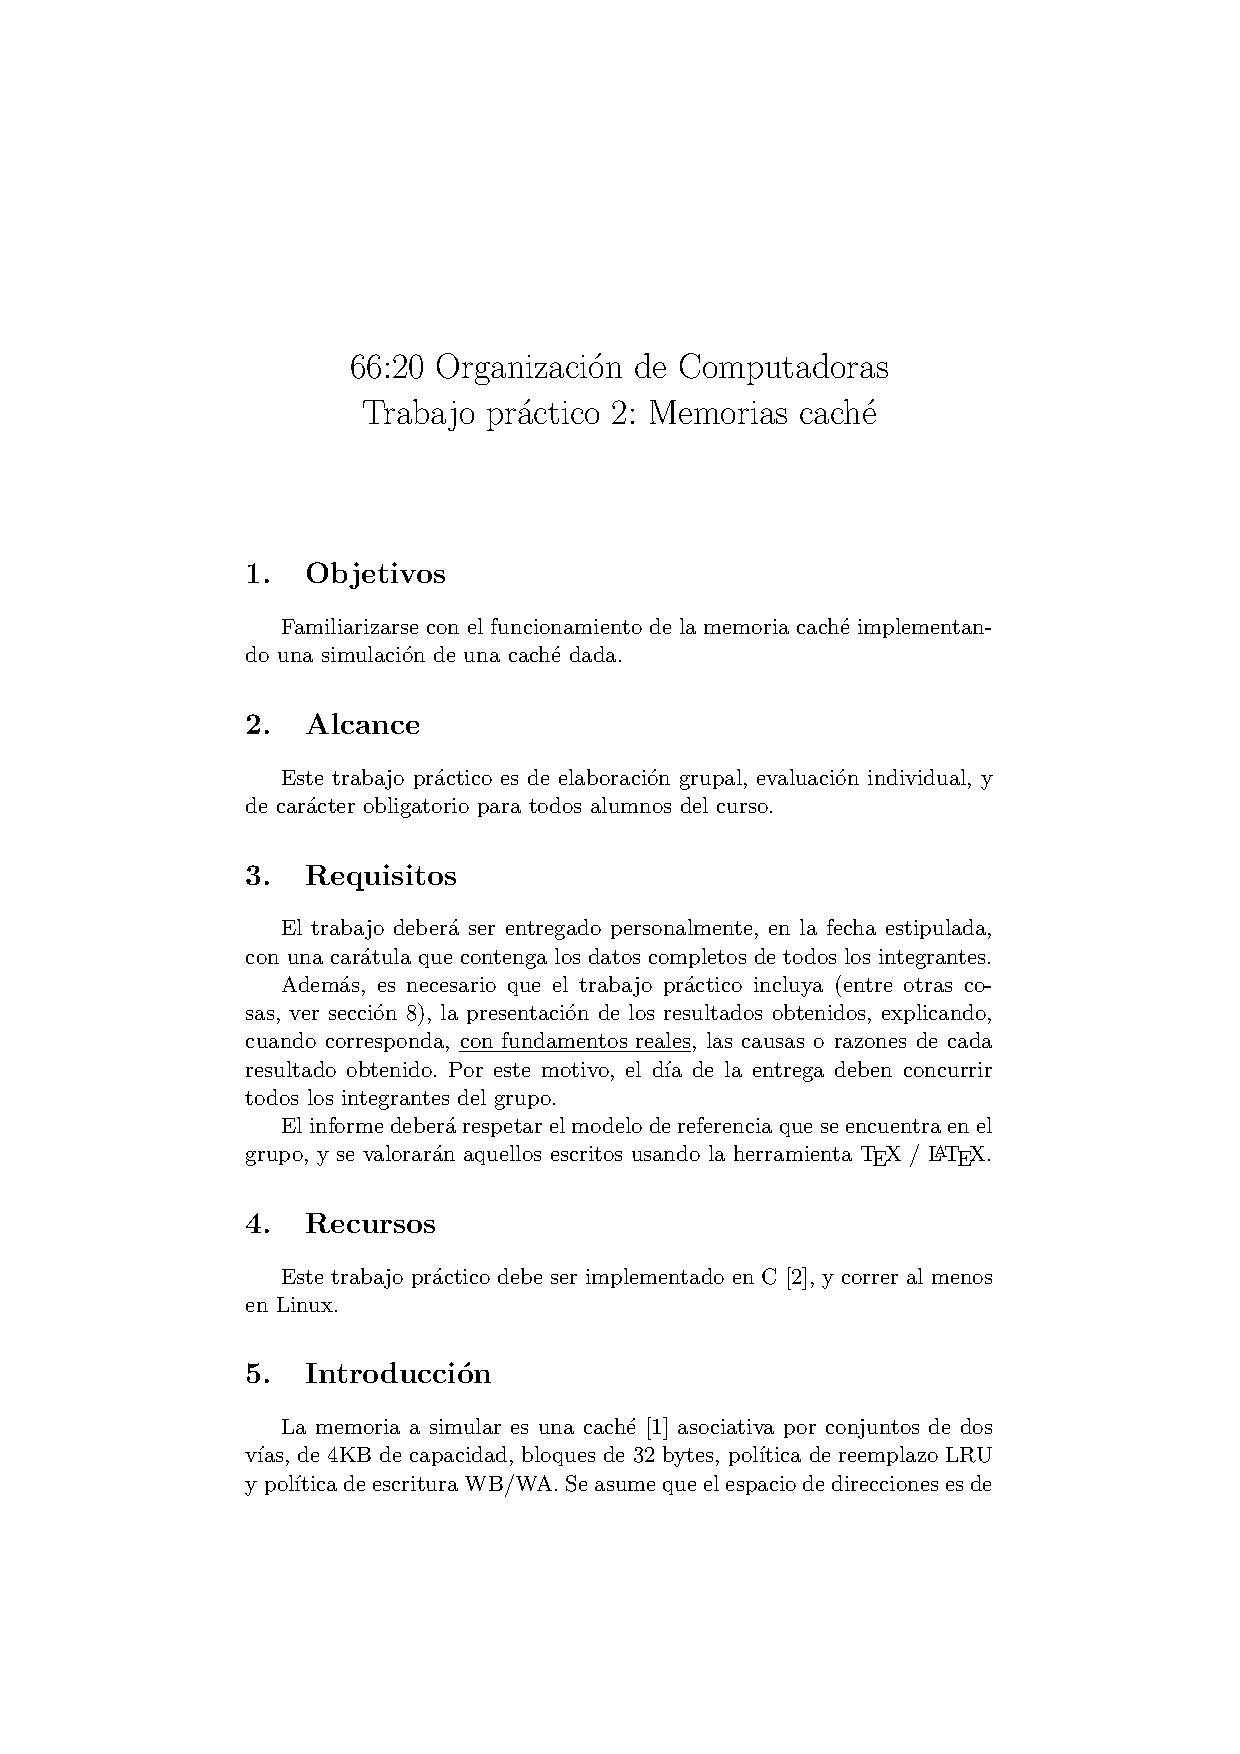
\includepdf[pages={1-}]{enunciado.pdf}

\end{document}
